% $Id$

\chapter{Removing confounds: a regression example}
\label{sec:confounds_reg}
\minitoc

\section{Introduction}

This chapter will describe the steps necessary to remove confounding effects using PRoNTo in a regression approach. These are similar to the ones used in the previous chapter, thus, the reader is advised to complete the tutorial in Chapter \ref{sec:confounds_clas} before moving on, since the explanation of some steps will be less descriptive. The dataset used in this chapter can be found on PRoNTo's website \url{http://www.mlnl.cs.ucl.ac.uk/pronto/prtdata.html} (data set 3).


As in previous Chapters, we will start analyzing the data with the PRoNTo's GUI and then repeating the analysis using the {\tt matlabbatch}  system. Please create a folder in your computer to store the results and type

\section{GUI analysis}

We will first analyse the data using PRoNTo's GUI and then repeat the analysis using the {\tt matlabbatch} system, then start up MATLAB and type `prt’ or `pronto’ in the MATLAB prompt. This will open the main interface of PRoNTo (see Figure \ref{fig:mainInterface} in Chapter \ref{sec:Block_design_fMRI_dataset}).

%--------------------------------------------------------------------------
\subsection{Data \& Design}

\begin{itemize}
	
	\item In PRoNTo's main window, click on `Data \& Design' 
	and a new window will open, `Data and design' (Figure \ref{fig:dataDesign}). Like in previous chapters, browse the directory in which to save the PRT structure (saved as `PRT.mat'); 
	
	\item In the panel ‘Groups’, click on ‘Add’ and provide a name to the group, e.g. `Aged'. 
	
	\item All the images in the dataset correspond to different subjects; therefore, click on the ‘Scans’ tick box. This will lock the ‘Subjects/Scans’ field, allowing you to skip to the third field. See Chapter \ref{sec:Block_design_fMRI_dataset} of the manual for more information on this option; 
	
	\item In the `Modalities' panel, click on `Add' and provide a name to the modality, e.g. `MRI'.
	
	\item Load all the image files available in the directory (IXIdata/aged/Guys/). You can select all the files by using the right mouse button and clicking on the option `Select All'. When all the images are selected, click on the `Done' button;
	
	\item In the `Covariates' field, type the covariates you want to regress out. In this example, `Gender' is the one chosen. As in the previous chapter, covariates can be input to PRoNTo by directly copying values into the Covariate if there is only one confounding factor, or by typing the full path of the R matrix containing either one column or multiple columns;
	
	\item In the `Regression targets' field, write (or paste) the list of target values available in the `Age\_old\_Guys' file (IXIdata/aged/), or input the full path of a rt\_subj.mat file containing the target values in a column. The final window should look like to the Figure \ref{fig:covariates_reg}. Press `OK'; 
	
	\begin{figure}[!h]
	\centering
		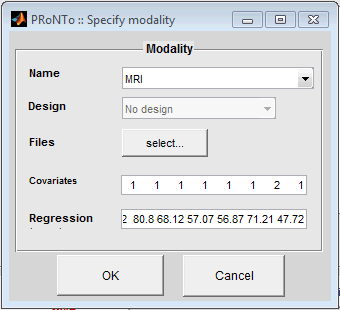
\includegraphics[scale=0.7]{images/Tutorial/confounds/covariates_regression.png}
	\caption{`Specify modality' GUI allows one to enter the covariates to be regressed out.}
	\label{fig:covariates_reg}
	\end{figure}
	
	\item In the `Masks' field, on the bottom left of the `Data and design' window, select the `mergedsmwrc1\_mask\_01' mask for the modality specified (Figure 12.6);
	
	\item The `Data and design' window should look similar to Figure \ref{fig:data_and_design_reg}. Click on the `Save' button to create `PRT.mat' file with the structure containing the information that has been previously specified. If no errors are shown in the MATLAB command, leave the `Data and design' window by clicking `Quit'.

\begin{figure}[!h]
	\centering
		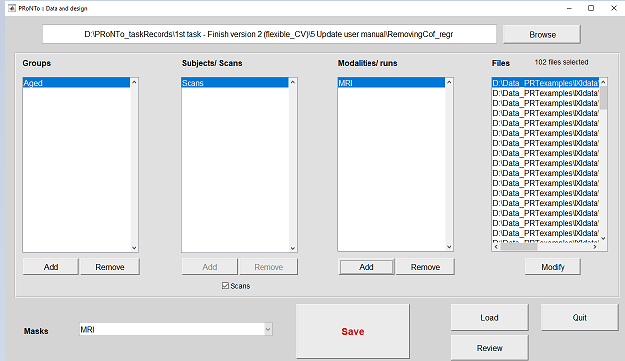
\includegraphics[scale=0.7]{images/Tutorial/confounds/Data_and_design_reg.png}
	\caption{`Data and design' GUI final configuration..}
	\label{fig:data_and_design_reg}
\end{figure}

\end{itemize}

%--------------------------------------------------------

\subsection{Prepare feature set}

\begin{itemize}
	
	\item In PRoNTo's main window, click on `Prepare feature set' and a new window will open, `Prepare feature set' (see Figure \ref{fig:prepareFeature} in Chapter \ref{sec:Block_design_fMRI_dataset});
	\item Select the `PRT.mat' file previously created in the `Data \& Design' step and another window will open, `Specify modality to include' (see Figure \ref{fig:specifyModality} in Chapter \ref{sec:confounds_clas});

	%
%	\begin{figure}[!h]
%	\centering
%		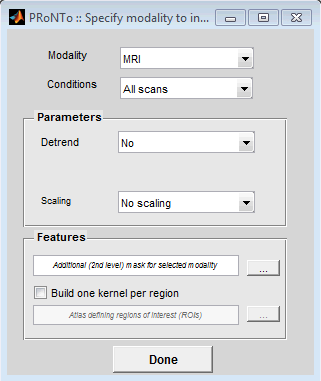
\includegraphics[scale=0.7]{images/Tutorial/confounds/specify_modality.png}
%	\caption{`Specify modality to include' GUI.}
%	\label{fig:specifyModality}
%	\end{figure}
		
	\item In the `Prepare feature set' window, provide a name for the feature set, e.g. `KRRAged';

	\item Click on `Build kernel/data matrix' to build the feature set and kernel.

\end{itemize}



%---------------------------------------------------------------------

\subsection{Specify model}

\begin{itemize}
	
	\item In PRoNTo's main window, click on `Specify model' and a new window will open, `Specify model' (see Figure \ref{fig:specifyModel} in Chapter \ref{sec:Block_design_fMRI_dataset});

	\item Select the `PRT.mat' file and provide a name to the model, e.g. `KRR';
	
	\item Select one of the `Feature Set' previously defined. In this case, there is only one:  `KRRAged';
	
	\item Leave the option `Use kernels' tick box as it is, i.e. `Yes';

	\item Select the `Regression' model type and click on the `Select subjects/scans` button. This will open a new window, `Specify subjects/scans to regress', click on the `Select all' button to use all the scans for the regression  (Figure \ref{fig:specifySubjects_reg});

	
\begin{figure}[!h]
	\centering
		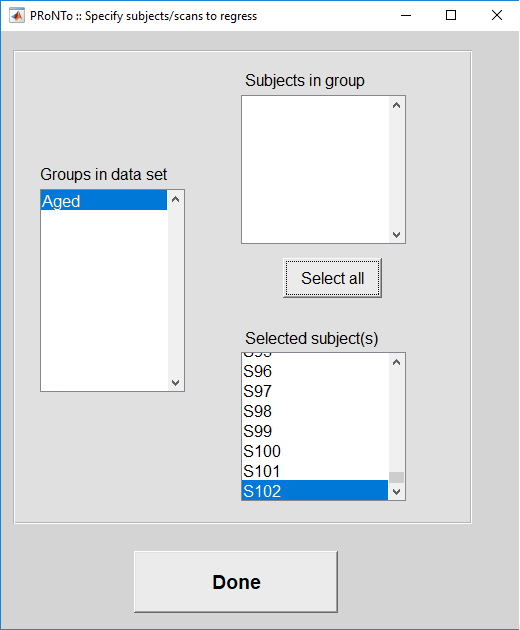
\includegraphics[height=9cm]{images/Tutorial/confounds/specify_subjects.png}
	\caption{`Specify classes' GUI.}
	\label{fig:specifySubjects_reg}
\end{figure}
	
	\item Select the `Kernel Ridge Regression' option, in the Machine field;	
	
	 \item Check the option `Optimize hyper-parameter' tick box (we will see later the importance of optimizing the hyperparameter when the confounds are removed). Type `10.\textasciicircum{}[-5:5]' on the right field. Then, select `k-fold CV on Subject-Out' option in the `Cross-Validation Scheme' field (internal loop). After that, type `5' in the new window that will open (see Figure \ref{fig:cv_reg});
	
		\begin{figure}[!h]
	\centering
		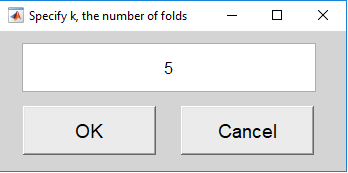
\includegraphics[scale=0.75]{images/Tutorial/confounds/cv_reg.png}
	\caption{Number of folds selected in the internal loop.}
	\label{fig:cv_reg}
	\end{figure}
	
	\item Select the `Leave One Subject Out' cross-validation scheme (external loop);
	
	\item In the `Data operations' box, select the `Regress out covariates (subject level)' option, which corresponds to the removal of the contribution of some external variables to the data, and `Mean centre features using training data' option. Then, the `Specify model' window should look similar to Figure \ref{fig:finalModel}. Click on the `Specify and run model' button;
	
	\begin{figure}[!h]
	\centering
		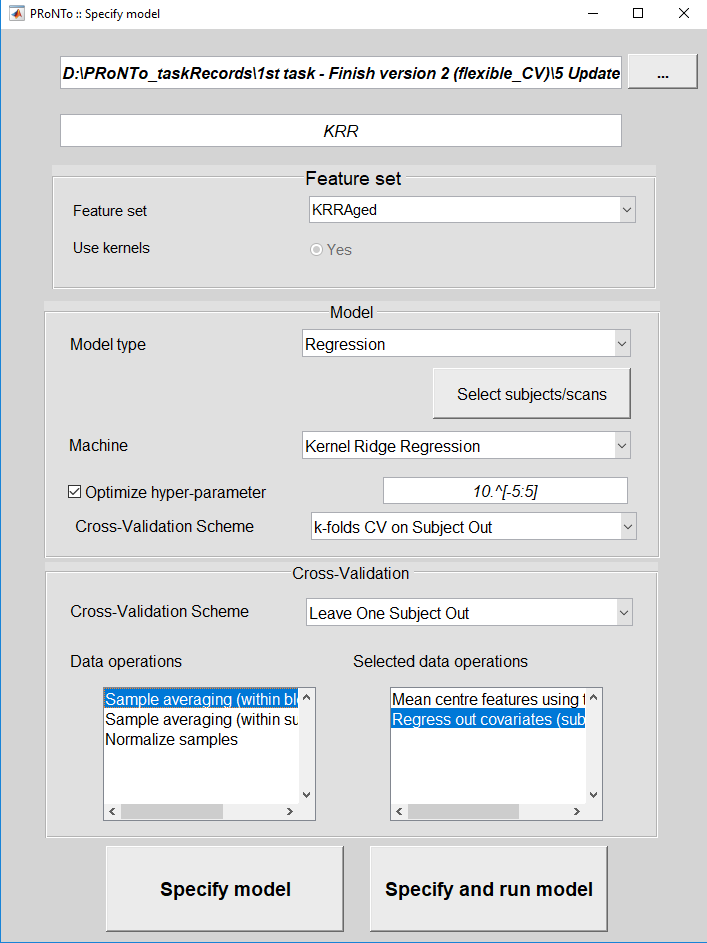
\includegraphics[scale=0.65]{images/Tutorial/confounds/specify_model_reg.png}
	\caption{`Specify model' GUI final configuration.}
	\label{fig:finalModel}
\end{figure}

	
\end{itemize}


%------------------------------------------------------------------

\subsection{Display results}
\label{display_results_confounds}

\begin{itemize}
	
	\item In PRoNTo's main window, click on `Display results' and select the `PRT.mat' file. This will open the main results window (Figure \ref{fig:results_reg});
	
\begin{figure}[h!]
	\centering
		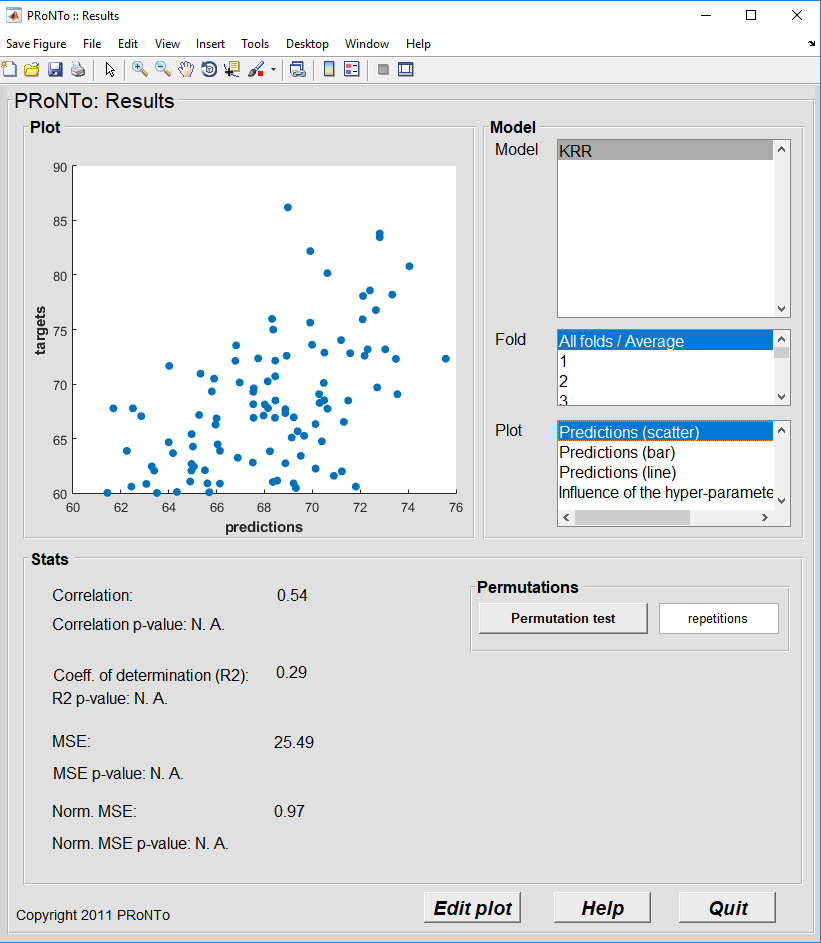
\includegraphics[scale=0.65]{images/Tutorial/confounds/results_reg.png}
	\caption{`Results' GUI.}
	\label{fig:results_reg}
\end{figure}

%\begin{figure}[h!]
%	\centering
%		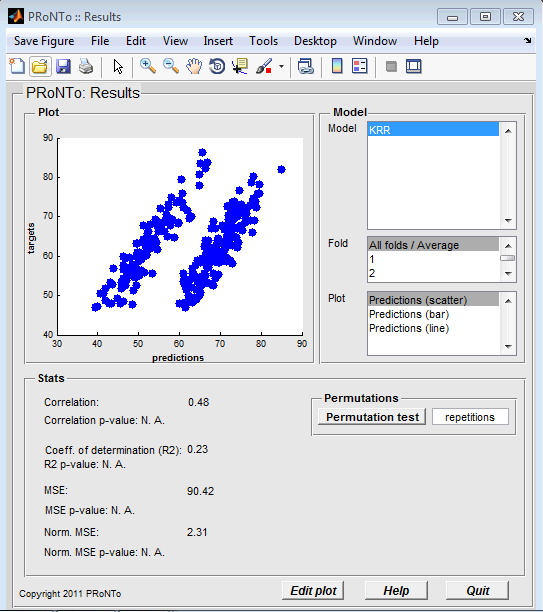
\includegraphics[scale=0.65]{images/Tutorial/confounds/results_no_opt.png}
%	\caption{`Results' GUI when the hyper-parameter is not optimized.}
%	\label{fig:results_no_opt}
%\end{figure}
	
	
   \item In the `Results' window, one can select the different regression models in the `Model' list on the upper right region. This will show the results obtained using each one of the regression models.

   \item It is important to optimize the hyperparameter when we try to remove confounds. From our experience, results without the hyperparameter optimization may be significantly different from results with hyperparameter optimization. But this effect may be data dependent. We therefore highly suggest users choose to perform this step. 
   %In Figure \ref{fig:results_no_opt} we can see the results when this operation is not done, where the different subjects are split according to their gender, getting two different regressions. 

\end{itemize}

%------------------------------------------------------------------


\subsection{Compute weights (optional step)}

\begin{itemize}
\item In PRoNTo's main window, click on `Compute weights' and a new window will open, `Compute weights' (Figure \ref{fig:weights_reg});

\begin{figure}[h!]
	\centering
		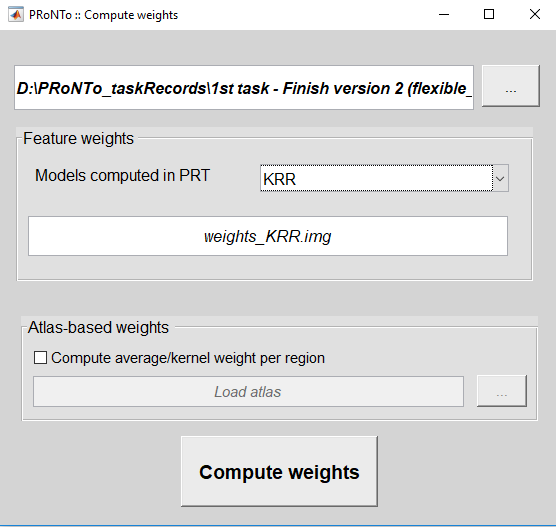
\includegraphics[scale=0.7]{images/Tutorial/confounds/weights_reg.png}
	\caption{`Compute weights' GUI.}
	\label{fig:weights_reg}
\end{figure}

\item Select the `PRT.mat' file;

\item Select the model from the list to `Models computed in PRT', `KRR' model;

\item Leave the option `Compute average/kernel weight per region' tick box unchecked;

\item Click on `Compute weights' button. Computations will be displayed on the MATLAB command window.

\end{itemize}
	

%=====================================================

\section{Batch analysis}
\label{sec:Batch_analysis_svm_confounds}

In this section, the previous experiment will be repeated using the `\texttt{matlabbatch}' system. The reader is advised to complete the tutorial in Section \ref{sec:Batch_analysis_svm} before continuing, since the explanation of each step will be less descriptive.

Once again, to analyse the data, create a new directory in which to save the results of the analysis. On the main interface of PRoNTo click on the `Batch' button to open the `{\tt matlabbatch}'. Alternatively, type `prt\_batch' in the MATLAB prompt.

%--------------------------------------------------------------

\subsection{Data \& Design}

\begin{itemize}

 	\item Click on `Data \& Design' in the PRoNTo menu (see Figure \ref{fig:batchData} in Chapter \ref{sec:Block_design_fMRI_dataset});	
	\item In the `Directory' field, select a directory where the `PRT.mat' file will be saved;
	
	\item In the `Groups' field:
 	
		\begin{itemize}
		
		\item Add one group;
		
		\item In the field `Name', provide a name without spaces for this group, e.g. `Aged';
		
		\item In the field `Select by', select the `Scans' option and add a new modality. For more information on the Scans option please consult Chapter \ref{chap:DataDesign};
		
		\item Provide a name for this modality, e.g. `MRI'; select the image files available in the `aged/Guys' directory of the IXI dataset and write (or paste) the regression targets\footnote{Available in the `Age\_old\_Guys' file (IXIdata/aged/)} in the `Regression targets (per scans)' field;
		
		\item Specify in the `Covariates' the file with the confounds you want to remove. Remember that this file should contain a variable `R' with a matrix of covariates (Data \& Design:Mod\#1 name) \footnote {It is possible to regress out more than one covariate just adding to the variable `R' as many columns as the number of covariates }. The batch editor should look similar to the Figure \ref{fig:Data_and_design_reg_batch};
		
		\begin{figure}[h!]
	\centering
		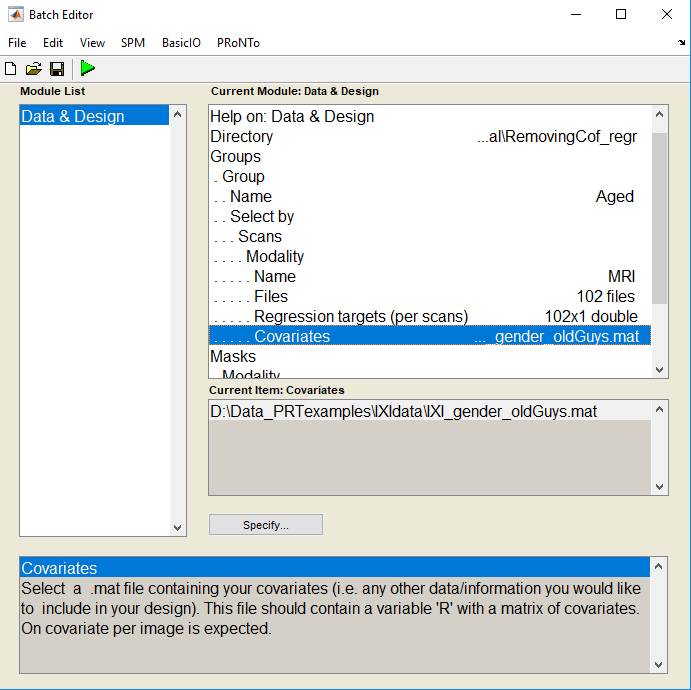
\includegraphics[scale=0.6]{images/Tutorial/confounds/Data_and_design_reg_batch.png}
	\caption{Data and design module in {\tt matlabbatch}. }
	\label{fig:Data_and_design_reg_batch}
	\end{figure}
				
		
	\end{itemize}
	
	\item In the `Masks' field, add a new modality and provide the same modality name, `fMRI'; and select the `whole\_brain' mask available in the masks directory of the Haxby dataset. The name of the modality here has to be exactly the same as in `Modalities', otherwise it will not work;
	
	%checar aqui
	
	\item Leave the `HRF overlap' and the `HRF delay' fields as default;
	
	\item In the `Review' field, select `Yes' if you would like to review your data and design in a separate window. Otherwise, leave as it is, i.e. `No'.


\end{itemize}

%------------------------------------------------------------

\subsection{Feature set / Kernel}

\begin{itemize}
	\item Click on the `Feature set / Kernel' option on PRoNTo's {\tt matlabbatch} menu (see Figure \ref{fig:batchFeature} in Chapter \ref{sec:Block_design_fMRI_dataset});
	
	\item With `Load PRT.mat' field selected, click on the `Dependency' button to associate the `PRT.mat' file created in the previous `Data \& Design' step (Figure \ref{fig:batchDependency}) or click on the `Select files' button to browse where `PRT.mat' file was saved;
	
	
    \item Provide a name to the `Feature/kernel' set, e.g. `KRRAged';
	
	\item Add one modality and select the modality name with the `Dependency' button\footnote{Or type it in manually, `MRI', but the name needs to be {\it exactly} the same as the one specified in the `Data \& Design' module.}(Data \& Design:Mod\#1 name);
	
		\begin{itemize}
	
	\item In the `Scans/Conditions' field , select the `All scans' option;
	
	\item In the `Voxels to include' field, select `All voxels' option, this means we are not entering an additional second-level mask;
	
	\item In the `Detrend' field, select `Polynomial detrend' option with order 1;
	
	\item In the `Scale input scans' field, select `No scaling' option;
	
	\item Leave `Load Atlas' as default. After all these steps, the batch editor should look similar to the one in Figure \ref{fig:feature_batch_reg};
	
	\begin{figure}[h!]
	\centering
		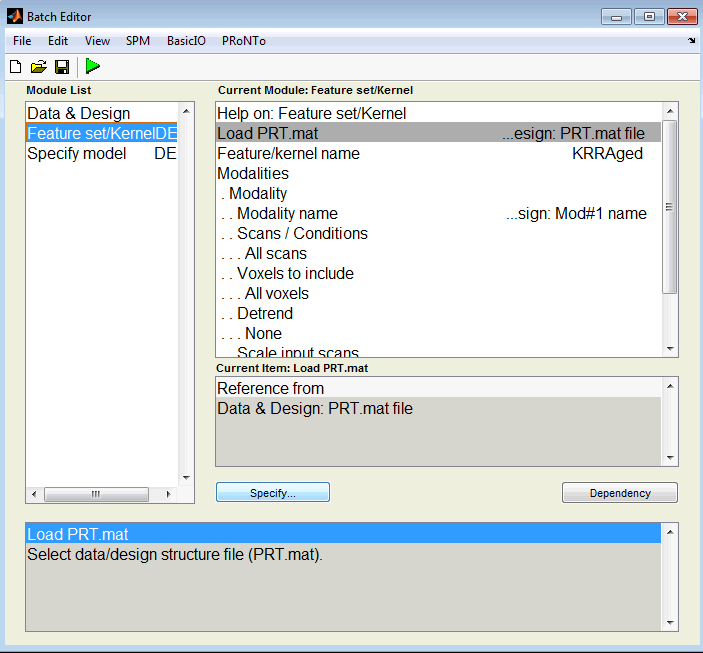
\includegraphics[scale=0.55]{images/Tutorial/confounds/feature_batch_reg.png}
	\caption{Feature set / Kernel module. Selected parameters in the Modality option.}
	\label{fig:feature_batch_reg}
\end{figure}
	
	\end{itemize}
	
	\item Leave the `Generate Multiple Kernels' and the `Use one kernel per modality' fields as default.
	

\end{itemize}

%--------------------------------------------------------

\subsection{Specify model}

\begin{itemize}

\item Click on the `Specify model' option on PRoNTo's {\tt matlabbatch} menu (see Figure \ref{fig:batchSpecifyModel} in Chapter \ref{sec:Block_design_fMRI_dataset});
	
\item With `Load PRT.mat' field selected, click on the `Dependency' button to associate the `PRT.mat' file created in the previous `Feature set / Kernel' step or click on the `Select files' button to browse where `PRT.mat' file was saved;

\item Provide a name to the model, e.g. `KRR';   

\item Leave the `Use kernels' field as it is, i.e. `Yes';    

\item Select the feature set name with the `Dependency' button\footnote{or write it {\it exactly} as previously defined in the `Feature set / Kernel' module (option `Feature set/Kernel: Feature/kernel name'), here `KRRAged'.};    
    
\item Select the `Regression' model type:
	
		\begin{itemize}
		
    		\item Add a new group and call it `Aged';
		
		   \item In the `Subjects' field, type `1:102'. This will instruct the program to use all the 102 scans, i.e. from scan 1 to scan 102;
		    \end{itemize}		
		
	\item In the `Machine' field:
	
	\begin{itemize}
   \item Select the `Kernel Ridge Regression' option:
	
	\item Change the `Optimize hyper-parameter' field as to `Yes'; Type `10.\textasciicircum{}[-5:5]' on the `Regularization' field. Then, select `k-fold CV on Subject-Out' option in the `Cross-Validation Scheme' field (internal loop).
	After that, type `5' in `k' field;
		
	\end{itemize}
	
	\item In the `Cross-validation type' field, select `Leave one subject out' option;
	
	\item Leave the `Include all scans' field as it is, i.e. `No';

	\item In the `Data operations' field: 
	
		\begin{itemize}
		\item  Leave the `Mean centre features' field as it is, i.e. `Yes'; 
				
		\item  Click on the `Other Operations' button, choose `Select operations', `New Operation' and select the `Regress out covariates (subject level)' option from the list. After all these steps, the batch editor should look similar to the one in Figure \ref{fig:model_batch_reg};
		\end{itemize}
		
	\begin{figure}[h!]
	\centering
		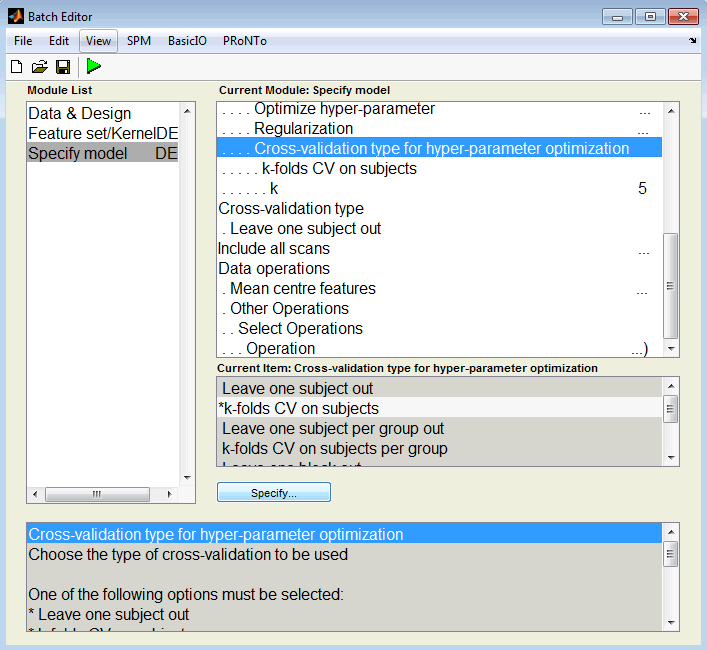
\includegraphics[scale=0.6]{images/Tutorial/confounds/model_batch_reg.png}
	\caption{Data and design module in {\tt matlabbatch}. }
	\label{fig:model_batch_reg}
	\end{figure}
	
\end{itemize}

%----------------------------------------------------------

\subsection{Run model}

\begin{itemize}

    \item Click on the `Run model' option on PRoNTo's {\tt matlabbatch} menu (see Figure \ref{fig:batchRun} in Chapter \ref{sec:Block_design_fMRI_dataset});
    
   	\item  With `Load PRT.mat' field selected, click on the `Dependency' button to associate the `PRT.mat' file created in the previous `Specify model' step;

    \item Select the model name from the `Specify model' module with the `Dependency' button\footnote{or write it {\it exactly} as previously defined in the `Specify model' module, here `KRR'};
    
    \item In the field `Do permutation test?', leave as it is, i.e. `No permutation test' 

\end{itemize}

